\Problem
{گام هشتم}
{
    مطابق آنچه در درس آموختیم برای حذف نویز از فیلتر استفاده کنیم.
    
    \begin{figure}[H]
        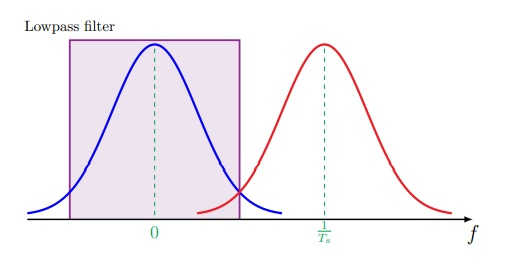
\includegraphics[]{Images/Filter.jpg}
        \centering
        \caption{تصویر خاکستری نویزی شده}
    \end{figure}
    
    برای حذف نویز از 4 فیلتر 
    \lr{wiener2}، \lr{filter2}، \lr{conv2} و \lr{medfilt2} 
    استفاده کردیم. سپس مقدار 
    \lr{SNR} و \lr{PSNR} را برای هر یک محاسبه کردیم.
    
    \begin{figure}[H]
        \centering
        \begin{minipage}[b]{0.4\textwidth}
            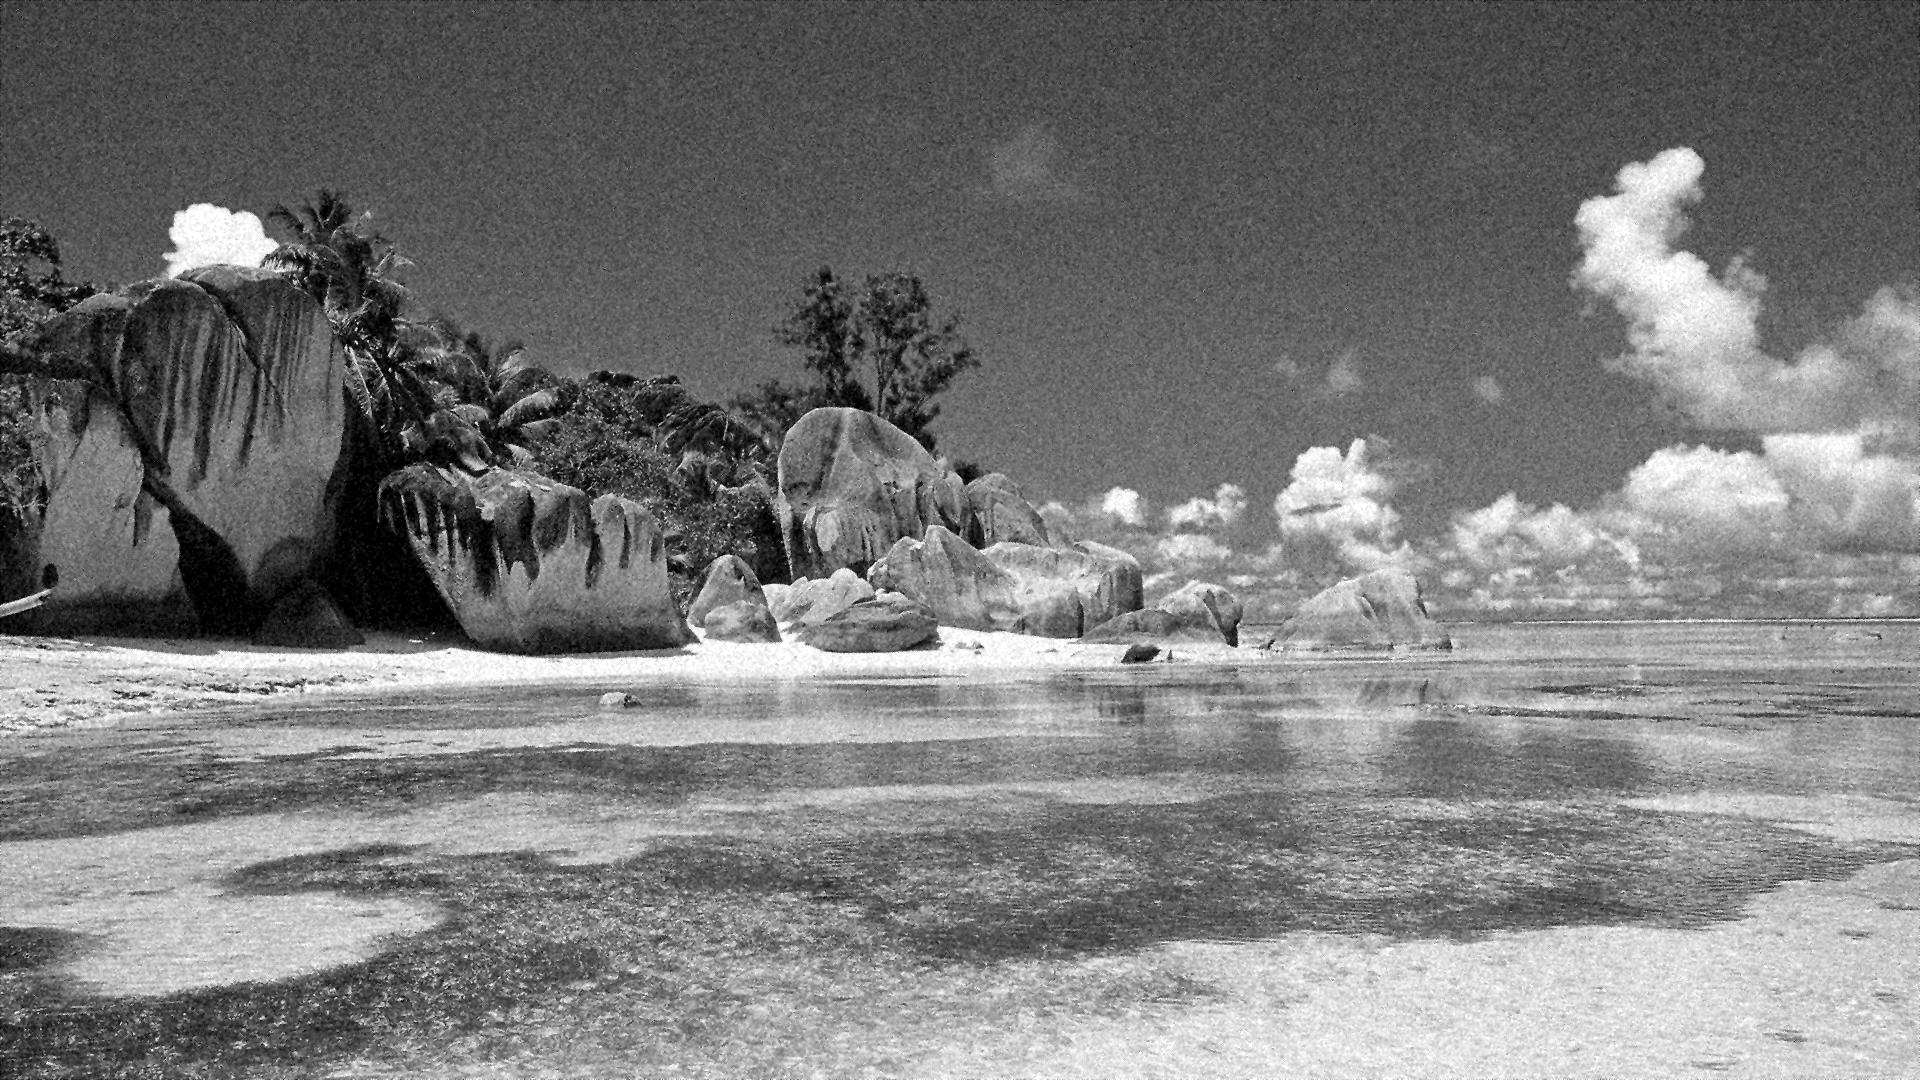
\includegraphics[width=\textwidth]{Images/Denoised_wiener.jpg}
            \caption{\lr{Wiener Filter}}
        \end{minipage}
        \begin{minipage}[b]{0.4\textwidth}
            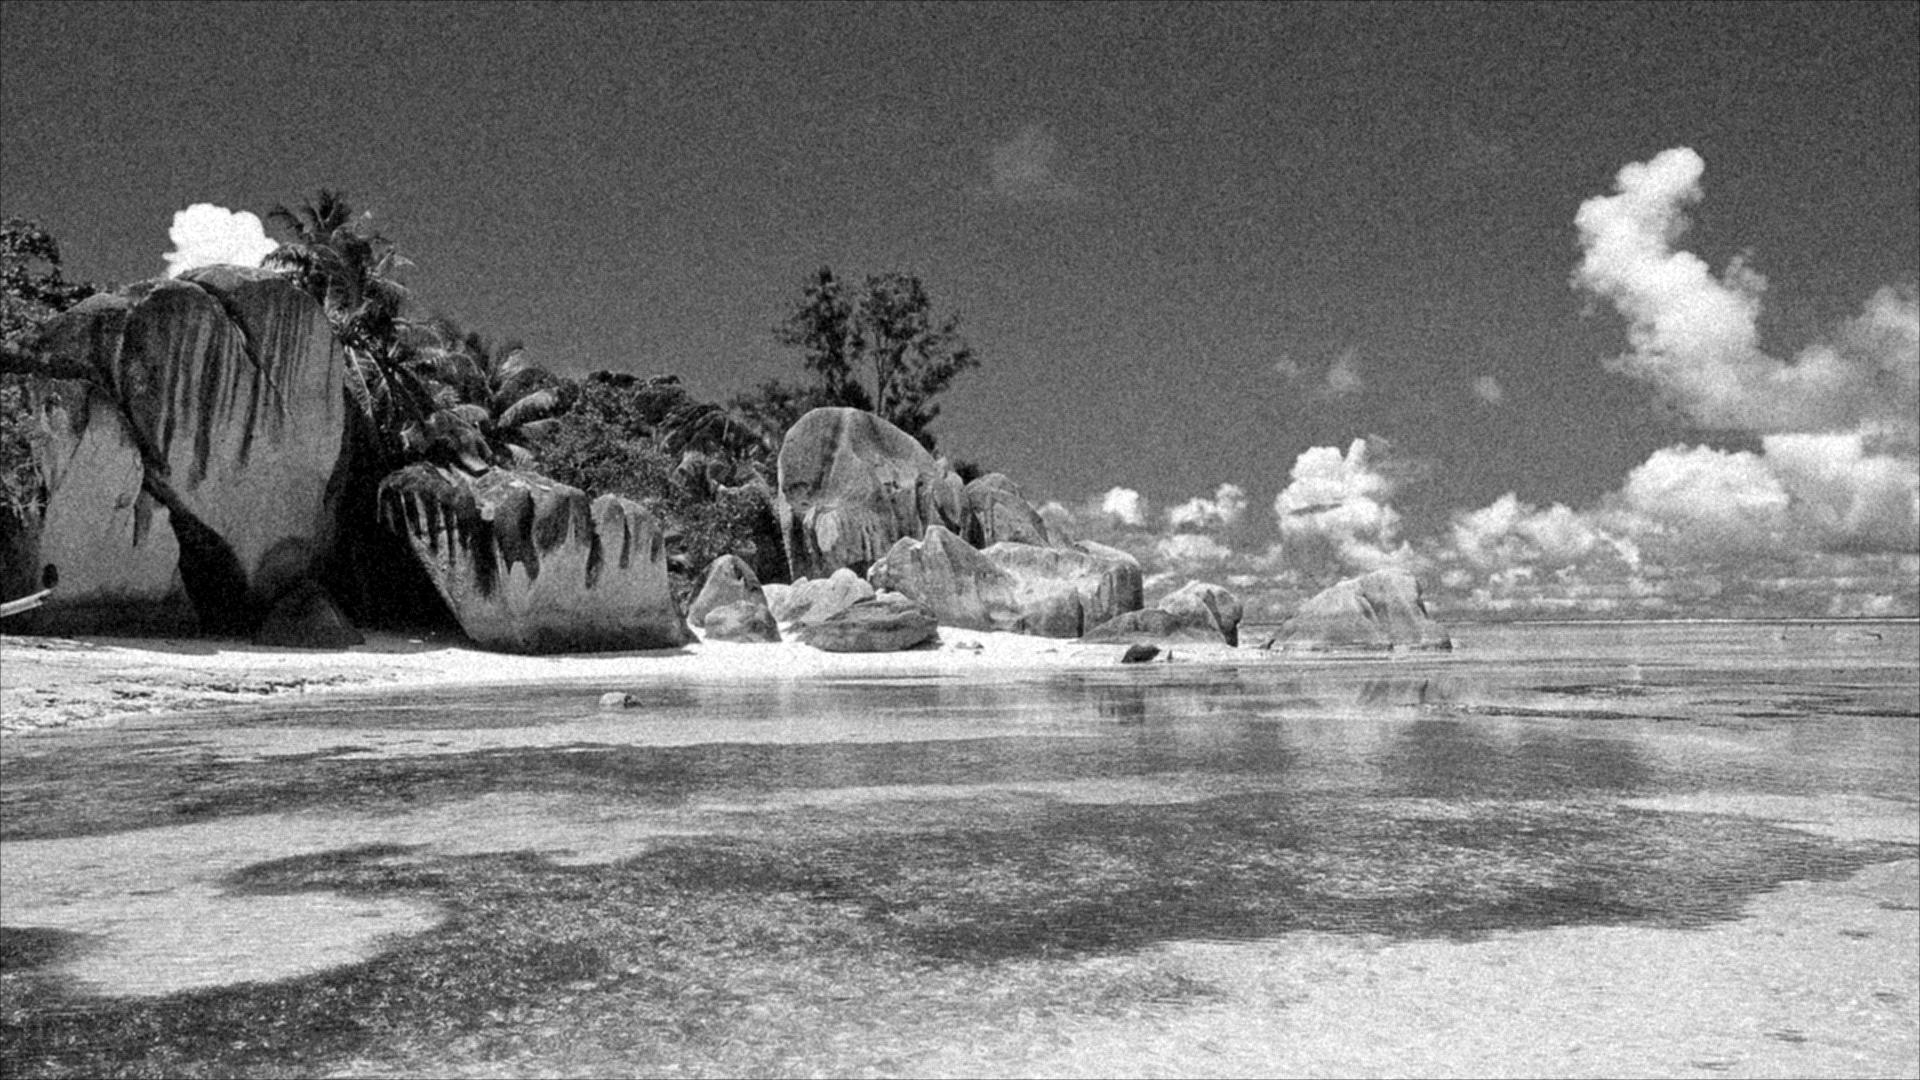
\includegraphics[width=\textwidth]{Images/Denoised_filter.jpg}
            \caption{\lr{Filter}}
        \end{minipage}
    \end{figure}
    
    \begin{figure}[H]
        \centering
        \begin{minipage}[b]{0.4\textwidth}
            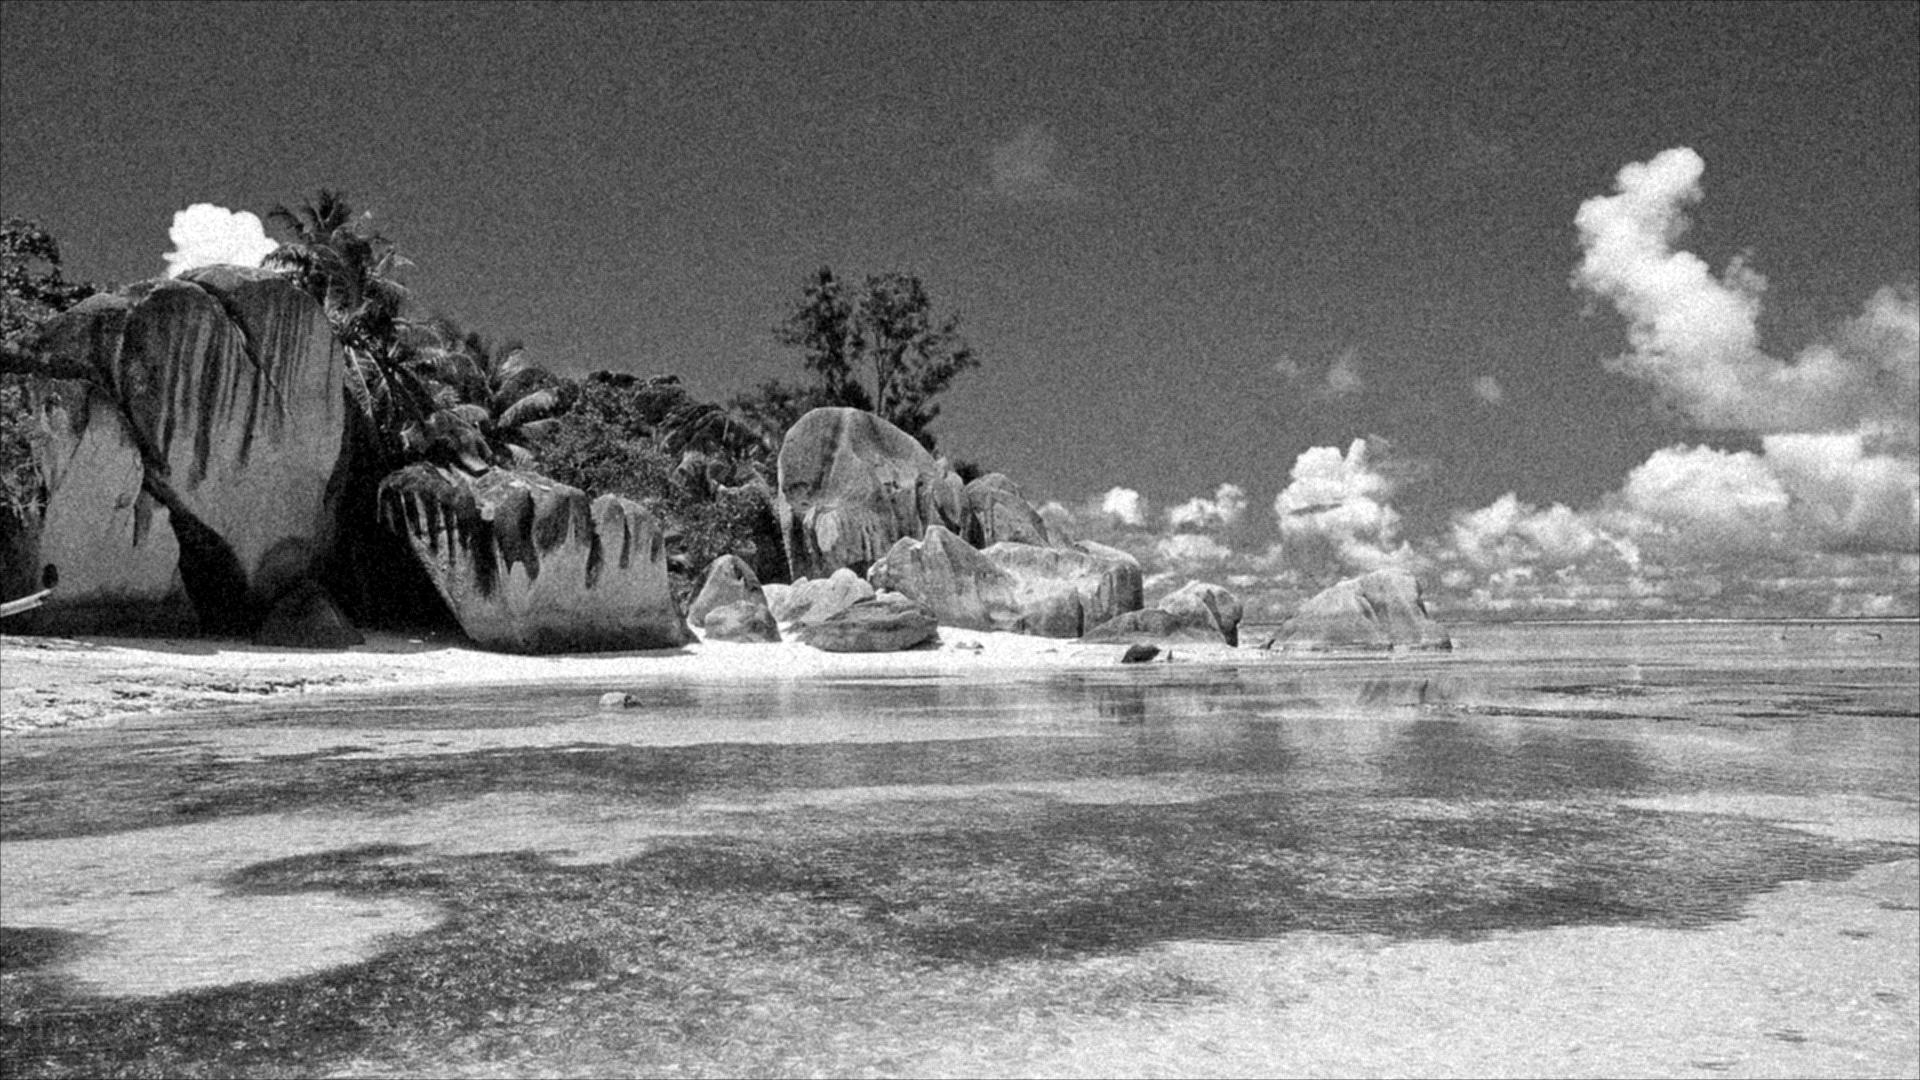
\includegraphics[width=\textwidth]{Images/Denoised_conv.jpg}
            \caption{\lr{Conv Filter}}
        \end{minipage}
        \begin{minipage}[b]{0.4\textwidth}
            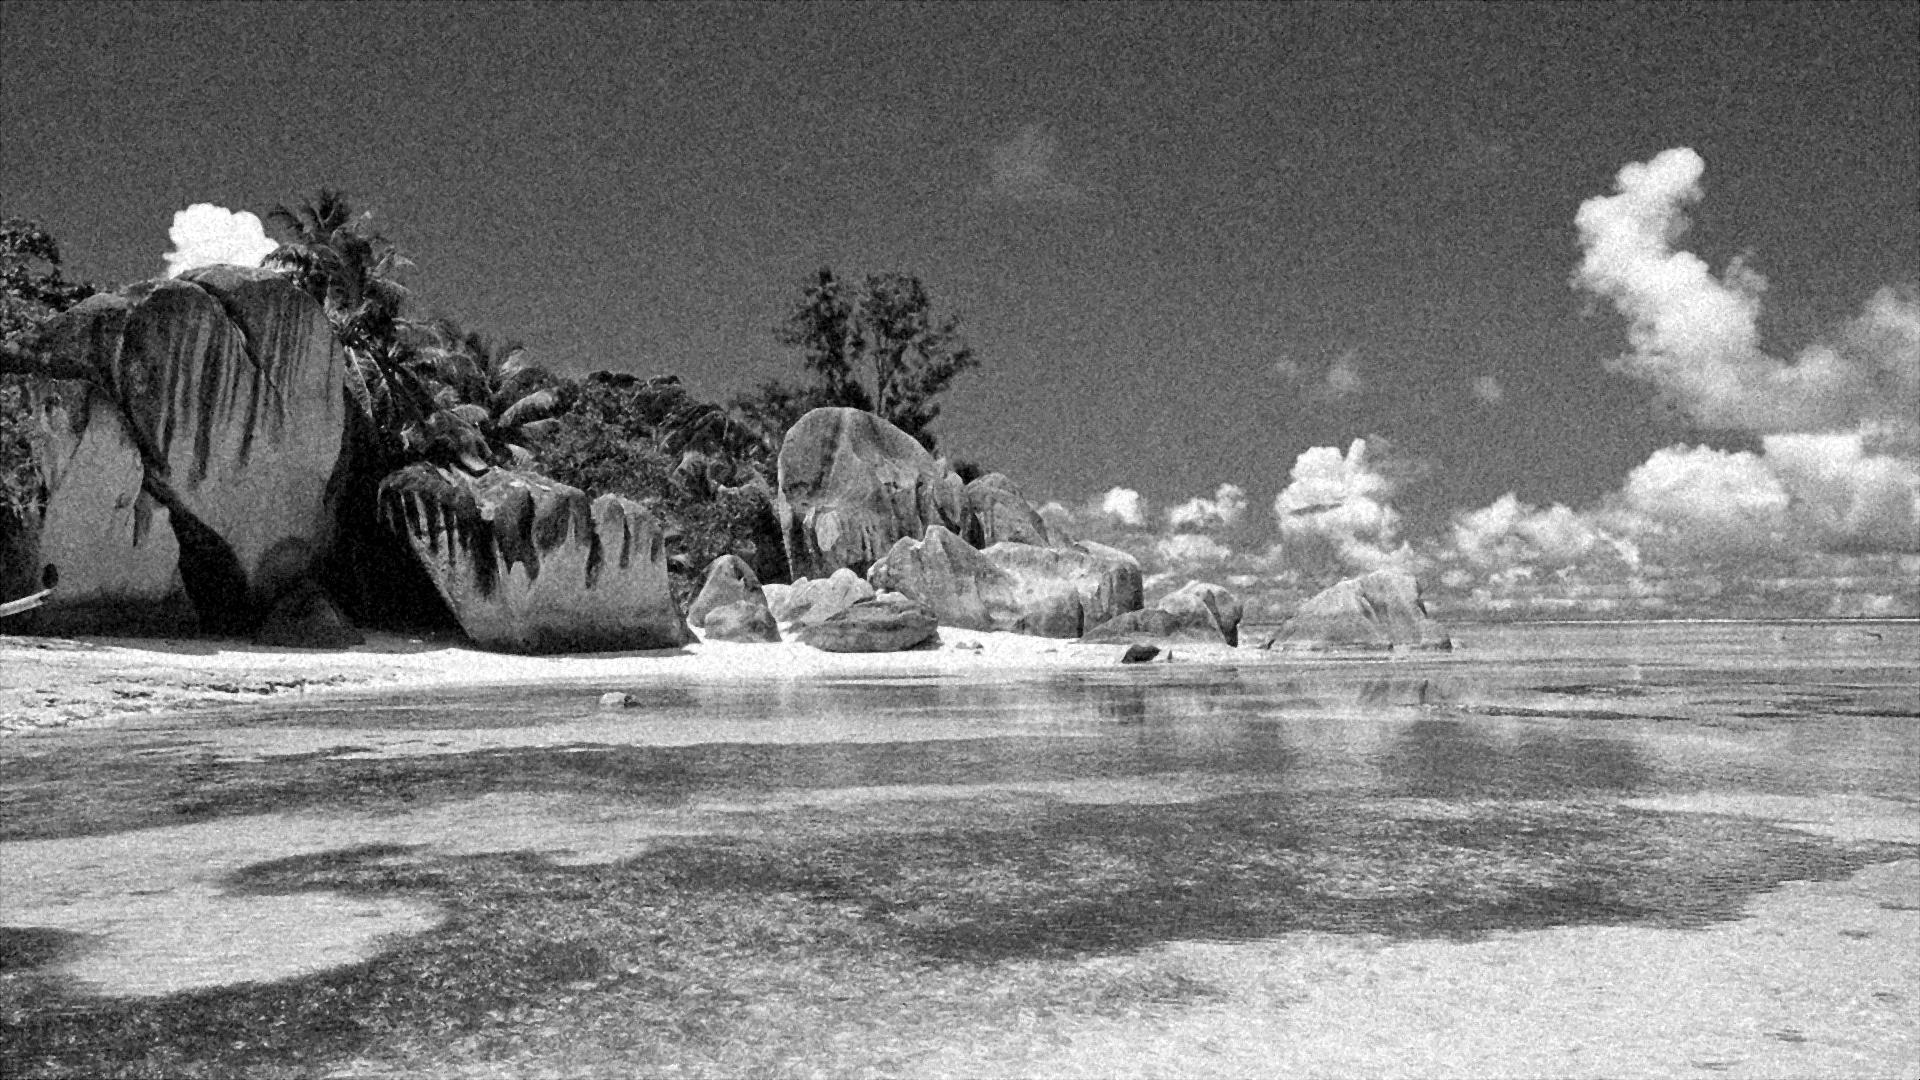
\includegraphics[width=\textwidth]{Images/Denoised_medfilt.jpg}
            \caption{\lr{Median Filter}}
        \end{minipage}
    \end{figure}
    
    \begin{figure}[H]
        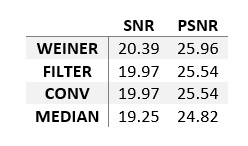
\includegraphics[]{Images/Table.jpg}
        \centering
        \caption{مقایسه انواع فیلتر‌ها}
    \end{figure}
    
    با توجه به مقادیر جدول می‌توان گفت:
    
    \begin{enumerate}
        \item فیلتر \lr{Weiner} بهترین عملکرد را داشته.
        \item دو فیلتر \lr{Conv} و \lr{Filter} عملکرد یکسانی دارند.
        \item فیلتر \lr{Median} بدترین عملکرد را دارد.
        \item پس از حذف نویز، نویز واقعا کاهش یافته است.
    \end{enumerate}
    
}
